%\documentclass[a4paper,12pt,final,twoside]{scrartcl}
\setcounter{secnumdepth}{3}
\setcounter{tocdepth}{5}

\usepackage[utf8]{inputenc}
\usepackage[T1]{fontenc}
\linespread{1.4}
\usepackage{dsfont}
\usepackage{amsfonts}
\usepackage{amsmath}
\usepackage{amssymb}
\usepackage{amsthm}
\usepackage{mathtools}
\usepackage{mathbbol}
\usepackage{amsmath1}
\usepackage[ngerman]{babel}
\usepackage{bibgerm}
\usepackage[pdftex]{graphicx}
%\usepackage{mathpazo}
\usepackage{floatflt}
%%\usepackage{epsfig}
\usepackage{wrapfig}
\usepackage{graphicx}
\usepackage{tabularx}
\usepackage{caption} 
\usepackage{multicol} 
\usepackage{mathrsfs}
%\usepackage{pspicture}
%\usepackage{eepic}
%\usepackage{epic}
%\usepackage{trfsigns}

%\usepackage[ansinew]{inputenc}
\usepackage{longtable,array,dcolumn}
%\usepackage{ngerman}
\usepackage{epic}
\usepackage{rotate}
\usepackage{graphpap}
\usepackage{amssymb}
\usepackage[squaren]{SIunits}
\usepackage{curves}
\usepackage{float}
\usepackage{array}
\usepackage{enumerate}
\usepackage{marvosym}
\usepackage{slashed}%für feynmanslsash
\usepackage[breaklinks,pdfborder={0 0 0}]{hyperref}
\usepackage{ulem}	%angeblich funktioniert dann
\let\underbar\uline	%underbar in math auch bei greek letters
\usepackage{multirow}
%\usepackage{multicolumn}
\usepackage{enumitem}


\setlength{\parskip}{12pt}
\setlength{\parindent}{0mm}
%\newcommand{\grad}{\ensuremath{^{\circ}}
%\renewcommand{\figurename}{Abb.}		% mit usepackage caption2
%\renewcommand{\captionfont}{\small \itshape}	% mit usepackage caption2
%\setkomafont{caption}{\small \itshape}		%sollte mit caption im userpackage funktionieren
%\setkomafont{captionlabel}{\small , \itshape}	%sollte mit caption im userpackage funktionieren
\captionsetup{font = {small, sf}} %mit it anstelle von sf gibts kusiv

\date{2009-20-10}
\newcommand{\kreis}[1]{
 \qbezier(-#1,0)(-#1,#1)(0,#1)
  \qbezier(0,#1)(#1,#1)(#1,0)
  \qbezier(#1,0)(#1,-#1)(0,-#1)
  \qbezier(0,-#1)(-#1,-#1)(-#1,0)}
\newcommand{\s}{\ \big| \ }
\newcommand{\lo}{\left <}
\newcommand{\ro}{\ri >}
\newcommand{\g}{&=&}

\newcommand{\ham}{\mathcal H}
\newcommand{\hil}{\mathscr H}
\newcommand{\fok}{\mathscr F}
\newcommand{\wh}{\widehat}
%\newcommand{\left}{\left}
\newcommand{\ri}{\right}
\newcommand{\Sp}{\text{Sp}}
\newcommand{\babsatz}{\par \begingroup \leftskip=2cm}
\newcommand{\eabsatz}{\par\endgroup}

\newcommand{\D}{\text{\itshape D}}
\newcommand{\Lr}{\mathcal L }%\textit{L}}
\newcommand{\rot}{\text{rot}}
\newcommand{\divergenz}{\text{div}}
\newcommand{\grad}{\text{grad}}
\newcommand{\grat}{${}^{\circ}$}
%\newcommand{\tanh}{\text{tanh}} already defined

\newcommand{\RM}[1]{\text{\MakeUppercase{\romannumeral #1}}}
\newcommand{\dell}{\partial}
\renewcommand{\div}{\operatorname{div}}
\newcommand{\I}{\dot{\text{\i\!\i}}}
\newcommand{\e}{\mathrm{e}}
\newcommand{\ket}[1]{\mid\!\!\!\,\,{#1}\rangle}
\newcommand{\bra}[1]{\langle{#1}\!\!\!\,\,\mid}
\newcommand{\braket}[2]{\langle{#1}\!\!\!\,\,\mid\!\!\!\,\,{#2}\rangle}
\newcommand{\bracket}[3]{\langle{#1}\!\!\!\,\,\mid\!\!\!\,\,{#2}\!\!\!\,\,\mid\!\!\!\,\,{#3}\rangle}
\newcommand{\1}{\mathds{1}}
\newcommand{\EW}[1]{\langle\!\!\,\,#1\!\!\,\,\rangle}
\newcommand{\arrowbox}[1]{-\!\!\!\!\:\text{(#1)}\!\!\!\;\;\!\!\!\rightarrow}

\newcommand{\ketI}[1]{\ket{#1}_{\!\!\;\text{I}}}
\newcommand{\ketII}[1]{\ket{#1}_{\!\!\;\text{II}}}
\newcommand{\ketIII}[1]{\ket{#1}_{\!\!\;\text{III}}}
\newcommand{\braI}[1]{\,\!_{\text{I}\!\!\;}\bra{#1}}
\newcommand{\braII}[1]{\,\!_{\text{II}\!\!\;}\bra{#1}}
\newcommand{\braketI}[2]{\,_{\text{I}\!\!\;}\braket{#1}{#2}_{\!\!\;\text{I}}\,}
\newcommand{\braketII}[2]{\,_{\text{II}\!\!\;}\braket{#1}{#2}_{\!\!\;\text{II}}\,}
\newcommand{\braketIII}[2]{\,_{\text{III}\!\!\;}\braket{#1}{#2}_{\!\!\;\text{III}}\,}
\newcommand{\bracketI}[3]{\,_{\text{I}\!\!\;}\bracket{#1}{#2}{#3}_{\!\!\;\text{I}}\,}
\newcommand{\bracketII}[3]{\,_{\text{II}\!\!\;}\bracket{#1}{#2}{#3}_{\!\!\;\text{II}}\,}


\newcommand{\up}{\ket{\uparrow}}
\newcommand{\updg}{\bra{\uparrow}}
\newcommand{\down}{\ket{\downarrow}}
\newcommand{\downdg}{\bra{\downarrow}}
\newcommand{\upup}{\ket{\uparrow\uparrow}}
\newcommand{\updown}{\ket{\uparrow\downarrow}}
\newcommand{\downup}{\ket{\downarrow\uparrow}}
\newcommand{\downdown}{\ket{\downarrow\downarrow}}

\newenvironment{itemize1}{\begin{itemize}[leftmargin=5mm,itemsep=-1ex,topsep=-1ex]}{\end{itemize}}

%\usepackage[left=2cm,right=2cm,top=1cm,bottom=1cm,includeheadfoot]{geometry}

\usepackage{fancyhdr}
\pagestyle{fancy}{\fancyhf{}
\fancyhead[LO,RE]{\footnotesize \rightmark}
\fancyfoot[C]{\footnotesize -$\,$\thepage$\;$-}
\renewcommand{\headrulewidth}{0.4pt}
\renewcommand{\footrulewidth}{0pt}}

\fancypagestyle{plain}{\fancyhf{}
\renewcommand{\headrulewidth}{0.4pt}
\fancyfoot[C]{\footnotesize -$\,$\thepage$\,$-}}

\usepackage{titlesec}
\titleformat{\section}[display]{\sffamily\bfseries\Huge\center}{Kapitel \thetitle:}{1ex}{}{}
\newcommand{\kapitel}[2]{$\;$\vspace{-1.5cm} \section[#1]{#2} \rule{17cm}{0.4pt}\vspace{3cm}}
\titleformat{\paragraph}[hang]{\sffamily\bfseries}{\thetitle:}{0ex}{\vspace{-0.15cm}}{\vspace{0.5cm}}

\title{ \vspace{1.5cm}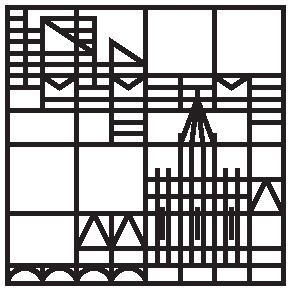
\includegraphics[width=5cm]{logo}
\\ \Large Universität Konstanz  \\ \vspace{4ex} \huge 
Skript zur Vorlesung\\ Höhere Quantentheorie und Elektrodynamik
\\ \vspace{4ex} \Large Prof. Dr. Wolfgang Belzig 
\\ Version vom 30. Juli 2012 \\ \vspace{4.5cm}
\normalsize Ursprünglichen Mitschrift von Birte Heinze im WS 09/10 \\ Ausführliche Überarbeitung von Tobias Lohse im WS 11/12 \vspace{-10cm}}
\author{}
\date{}
%\begin{document}

\subsection{Streutheorie}
Im folgenden Abschnitt soll die quantenmechanische Beschreibung von Streuprozessen näher beschrieben werden. Diese stellt einen der wichtigsten Anwendungsbereiche der Quantenmechanik dar, beispielsweise zur Bestimmung von Kernkräften oder Kristallstrukturen. Im Gegensatz  zu spektroskopischen Prozessen liegen bei Streuprozessen Anfangs- und Endzustand des betrachteten Systems im kontinuierlichen Teil des Eigenwertspektrums. Das gestreute Teilchen kommt aus dem Unendlichen in den Wirkungsbereich des Streukörpers, um nach dem Stoß asymptotisch detektiert zu werden. Es befindet sich also nicht in einem gebundenen Zustand. 

Im Gegensatz zur klassischen Streutheorie kann die Quantenmechanik nur  stochastische Aussagen über das Ergebnis der Ergebnis der Streuung machen. Insbesondere ist der Wirkungsquerschnitt des Streuprozesses, der sogenannte {\bf Streuquerschnitt}, interessant, welcher die Wahrscheinlichkeit angibt mit der ein Teilchen in einen bestimmten Raumwinkel $\Omega=(\vartheta,\varphi)$ gestreut wird. Der Streuquerschnitt kann direkt experimentell bestimmt werden, indem ein Teilchenstrahl auf den zu untersuchenden Streukörper gelenkt wird und mit einem Detektor der Teilchenstrahl nach der Streuung in allen Raumwinkeln abgetastet wird. Aus diesen Daten können dann Rückschlüsse auf die Struktur des Streukörpers gezogen werden, sofern der Zusammenhang zwischen dem Wirkungsquerschnitt und den elementaren Wechselwirkungspotentialen bekannt ist. Dieser Aufgabe wollen wir uns im folgenden zuwenden. 


\subsubsection{Streuung eines Wellenpakets}

Es soll zunächst die Ablenkung eines einlaufenden freien Teilchens, welches durch ein ebenes Wellenpaket beschrieben wird, an einem lokalisierten Potential beschrieben werden. Die folgende Abbildung soll diesen Prozess veranschaulichen: 
\vspace{-2ex}\begin{figure}[!h]\center
	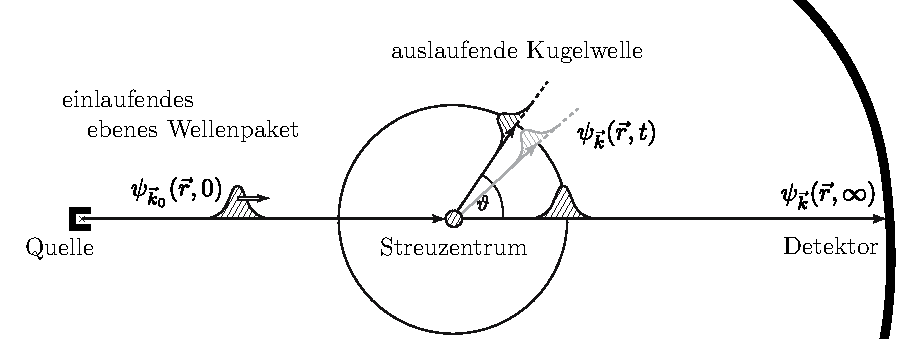
\includegraphics[scale=1]{Figs/Streuung}
\end{figure}\vspace{-4ex} 

Ein ebenes Wellenpaket $\psi_{\vec{k}_0}(\vec{r},0)$ mit Geschwindigkeit $\hbar\vec{k}_0/m$ trifft auf ein lokalisiertes Potential $\hat{V}$. Der Wechselwirkungsbereich dieses Potentials $\hat{V}(\vec{r})\neq0$ ist relativ klein, so dass wir es uns als relativ kleines Streuzentrum vorstellen können. Das Wellenpaket wechselwirkt nun also mit dem Potential und wird zu $\psi_{\vec{k}}(\vec{r},t)$, welches sich zusammensetzt aus einem Teil des Wellenpakets $\psi_{\vec{k}_0}(\vec{r},0)$ welches mit geringerer Intensität weiter läuft und einem anderer Teil, welcher asymptotisch als Kugelwelle beschrieben werden kann. Durch einen weit entfernten Detektor wird dann das Wellenpaket $\psi(\vec{r},\infty)$ detektiert. 

Das System wird durch den Hamiltonoperator $\hat{\ham}=-\hbar^2/2m\cdot\triangle + \hat{V}(\vec{r})$ beschrieben. Das einfallende Wellenpaket zur Zeit $t=0$ lässt sich wie folgt beschreiben:
\begin{eqnarray*}
	\psi_{\vec{k}_0}(\vec{r},0) &=& \int \frac{\mathrm{d} ^3k}{(2\pi)^3}\cdot \e^{\;\I\vec{k}\vec{r}}\cdot a_{\vec{k}} 
\end{eqnarray*}
Dabei haben die $a_{\vec{k}}$ ein Maximum bei $\vec{k}=\vec{k}_0$ und  $\e^{\;\I\vec{k}\vec{r}}$ sind die Eigenzustände des ungestörten Hamiltonoperators $\hat{\ham}_0=-\hbar^2/2m\cdot\triangle$ mit den Eigenwerten $E_{\vec{k}}=\hbar^2k^2/2m$. Die Eigenzustände $\psi_{\vec{k}}(\vec{r})$ des vollständigen Hamiltonoperators mit denselben Energien $E_{\vec{k}}$ sind durch die stationäre Schrödingergleichung (\ref{statSG}) bestimmt: 
\begin{eqnarray*}
	\Big(\frac{\hbar^2}{2m}\cdot\triangle + E_{\vec{k}}\Big)\;\psi_{\vec{k}}(\vec{r}) &=& \hat{V}(\vec{r})\;\psi_{\vec{k}}(\vec{r})
\end{eqnarray*}
Die Entwicklung des Eigenzustands $\psi_{\vec{k}_0}(\vec{r},0)$ nach $\psi_{\vec{k}}(\vec{r})$ liefert somit folgendes:
\begin{eqnarray*}
	\psi_{\vec{k}_0}(\vec{r},0) &=& \int \frac{\mathrm{d}^3 k}{(2 \pi)^3}\cdot \psi_{\vec{k}}(\vec{r})\cdot a_{\vec k}
\end{eqnarray*}
Wegen der asymptotischen Form $\e^{\;\I\vec{k}\vec{r}}$ der $\psi_{\vec{k}}(\vec{r})$ sind die $a_{\vec{k}}$ die selben für beide Darstellungen von $\psi_{\vec{k}_0}(\vec{r},0)$. Das heißt es kommen keine gebundenen Zustände vor, denn diese würden per Definition für $|\vec{r}| \to \infty$ verschwinden. 

Die Zustände zu einem beliebigen späteren Zeitpunkt $t>0$ ergeben sich für den zeitunabhängigen Hamiltonoperator direkt zu: 
\begin{eqnarray*}
	\psi(\vec{r},t) = \int \frac{d^3 k}{(2\pi)^3}\cdot\psi_{\vec{k}}(\vec{r})\cdot a_{\vec k} \cdot \e^{-\frac{\I}{\hbar}\cdot  E_{\vec{k}} t}
\end{eqnarray*}
Die Koeffizienten $a_{\vec{k}}$ sind dabei näherungsweise dieselben, wenn $\psi(\vec{r},0)$ vollständing außerhalb des Potentials liegt und $\psi_{\vec{k}}(\vec{r})\approx \e^{\I kr}$ gilt. 

Die Zeitentwicklung ist also mit der obigen Gleichung beschrieben, soll hier aber noch einmal anschaulich beschreiben werden. Nach der Streuung läuft einerseits das Wellenpaket mit geringerer Intensität weiter und andererseits läuft eine gestreute Kugelwelle aus, die jedoch eine winkelabhängige Amplitude besitzt.


\subsubsection{Formale Lösung der zeitunabhängigen Schrödingergleichung}\label{sec3.2}

Wir wollen nun die Form der $\psi_{\vec{k}}(\vec{r})$ bestimmen. Dazu müssen wir eine allgemeine Lösung der stationären Schrödingergleichung finden. Da das Potential in unserem Fall üblicherweise im Ortsraum nur eine einfache Funktion darstellt $\hat{V}(\vec{r})=V(\vec{r})$, hat die Gleichung die Form einer stationären Wellengleichung mit einer Inhomogenität: 
\begin{eqnarray}
	\Big( \frac{\hbar^2}{2m}\cdot \triangle + E_{\vec{k}}\Big)\;\psi_{\vec{r}}(\vec{r}) &=& V(\vec{r}) \cdot\psi_{\vec{k}}(\vec{r}) \label{statSGwelle}
\end{eqnarray}
Eine solche Gleichung lässt sich mit Hilfe der retardierten {\bf Greenschen Funktion} $G_{\vec{k}}(\vec{r}-\vec{r}\,')$ lösen. Die Greensche Funktion der Wellengleichung ist definiert als: 
\begin{eqnarray*}
	\Big( \frac{\hbar^2}{2m}\cdot\triangle + E_{\vec{k}}\Big)\; G_{\vec{k}}(\vec{r}- \vec{r}\,') &=& \delta(\vec{r} - \vec{r}\,')
\end{eqnarray*}
Diese Eigenwertgleichung ist mittels Fourier-Transformation einfach zu lösen. Es ergibt sich folgende explizite Darstellung der Greenschen Funktion:
\begin{eqnarray*}
	G_{\vec k}(r) &=& -\frac{m}{2\pi \hbar^2} \cdot \frac{e^{i k r}}{r}
\end{eqnarray*}
Die Greensche Funktion hat wie vermutet die Form einer auslaufenden Kugelwelle. Wir können somit die Gleichung (\ref{statSGwelle}) in eine Integralgleichung umschreiben:
\begin{eqnarray*}
	\psi_{\vec{k}}(\vec{r}) &=& \e^{\;\I\vec{k}\vec{r}} + \int\mathrm{d}^3 r'\; G(\vec{r}-\vec{r}\,')\cdot V(\vec{r}\,') \cdot\psi_{\vec{k}}(\vec{r}\,')
\end{eqnarray*}
Der Term $\e^{\;\I\vec{k}\vec{r}}$ ist die Lösung der homogenen Gleichung, er gewährleistet, dass die Anschlussbedingungen für asymptotisches Verhalten $|\vec{r}|\gg|\vec{r}\,'|$, erfüllt ist. In der Asymptotik gilt: 
\begin{eqnarray*}
	k \cdot |\vec{r}-\vec{r}\,'| = k \sqrt{r^2+r'\,^2-2\cdot\vec{r}\cdot\vec{r}\,'} \approx  k r \underbrace{\sqrt{1- \frac{2\cdot\vec{r}\cdot\vec{r}\,'}{r^2}}}_{\ll 1} \approx k r -\vec{k}_{\vec{r}}\vec{r}\,' \qquad \text{mit: } \vec k _{\vec r} = k \cdot \frac{\vec r}r
\end{eqnarray*}
Die folgende Skizze soll die Lage der Vektoren $\vec{k}$ und $\vec{k}_{\vec{r}}$ verdeutlichen. Wir können dabei $\vec{k}$ ohne Beschränkung der Allgemeinheit entlang der $z$-Achse legen: 
\begin{center}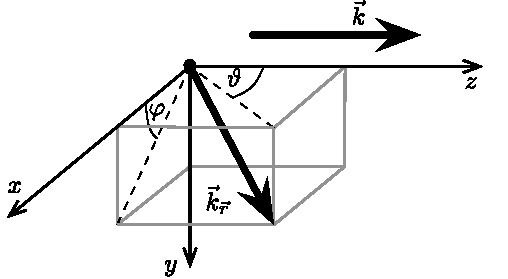
\includegraphics[scale=1]{Figs/kkr}\end{center}

Wir können somit die Welle $\psi_{\vec{k}}(\vec{r})$ in folgende Form umschreiben: 
\begin{eqnarray}
	\psi_{\vec{k}}(\vec{r}) = \e^{\;\I\vec{k}\vec{r}} + \frac{1}{r}\cdot f_{\vec{k}}(\vartheta,\varphi)\cdot\e^{\;\I kr} &\quad& \text{mit: } f_{\vec{k}}(\vartheta,\varphi) = -\frac{m}{2\pi\hbar^2} \int\mathrm{d}^3r'\;\e^{-\I\vec{k}_{\vec{r}}\;\vec{r}\,'}\cdot V(\vec{r}\,')\cdot \psi_{\vec{k}}(\vec{r}\,')\qquad\quad \label{streuzustand}
\end{eqnarray}
In dieser Form kann man nun gut erkennen, dass die ebene Welle hinter dem Streupotential mit geringerer Intensität weiterläuft und die gestreute Welle als Kugelwelle ausläuft, wobei die winkelabhängige Streuamplitude $f_{\vec{k}}(\vartheta,\varphi)$, die Information über das Potential enthält. Die Streuamplitude hängt dabei von der Richtung $(\vartheta,\varphi)$ der Beobachtung sowie von der Wellenlänge $\lambda=2\pi/k$ ab. Sie wird außerdem durch die exakten Lösung $\psi_{\vec k}(\vec r)$ der Schrödingergleichung bestimmt und hat die Dimension einer Länge. 


\subsubsection{Streuquerschnitt}

Wie bereits erwähnt ist der Streuquerschnitt eine wichtige Größe zur Beschreibung des Streuprozessen. Man Unterscheidet generell zwischen dem differentiellen und totalen Streuquerschnit. Der {\bf differentieller Streuquerschnitt} $\mathrm{d}\sigma/\mathrm{d}\Omega\;$ ist definiert als Quotient aus dem Strom der  pro Raumwinkel gestreuten Teilchen $\mathrm{d}I/\mathrm{d}\Omega$ und dem Betrag der Stromdichte der einfallenden Teilchen $j_{\text{ein}}$:
\begin{eqnarray*}
	\frac{\mathrm{d}\sigma}{\mathrm{d}\Omega} &=& \frac{\mathrm{d} I}{\mathrm{d}\Omega}\cdot\frac{1}{j_{\text{ein}}} \quad\!=\!\quad \frac{j_r\cdot r^2}{j_{\text{ein}}}
\end{eqnarray*}
Dabei ist $j_r$ der Betrag der Stromdichte der auslaufenden Kugelwelle. Zur Umformung wurde dabei die Kugelsymmetrie ausgenutzt, wegen der sich der infinitesimale Strom der ausfallenden Teilchen schreiben lässt als $\mathrm{d}I=\vec{j}_r\;\mathrm{d}\vec{A} = j_r\cdot r^2\;\mathrm{d}\Omega$. Die folgende Skizze soll die räumlichen Zusammenhänge etwas besser verdeutlichen: 
\vspace{-1ex}\begin{figure}[!h]\center
	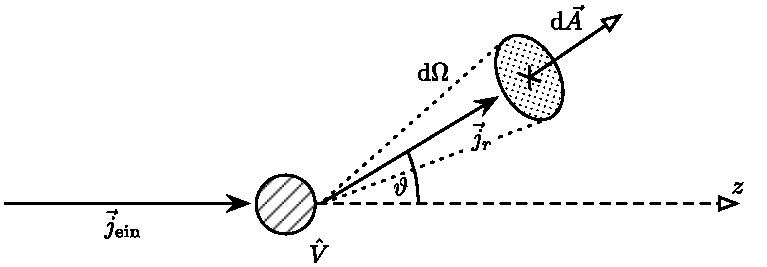
\includegraphics[scale=1]{Figs/DiffStreuQuer}
\end{figure}\vspace{-4ex} 

Die Stromdichte $j_{\text{ein}}$ der einfallenden Welle $\psi_{\vec{k}_0}(\vec{r},0)$ lässt sich berechnen zu:
\begin{eqnarray*}
	\vec{j}_{\text{ein}} &=& -\frac{\I\hbar}{2m}\cdot\big(\psi_{\vec{k}_0}^*\nabla\psi_{\vec{k}_0}-\psi_{\vec{k}_0}\nabla\psi_{\vec{k}_0}^*\big) \;=\; \frac {\hbar \vec{k}}{m}
\end{eqnarray*}
Der Betrag der Stromdichte $j_r$ der radial auslaufenden Kugelwelle $\psi_{\vec{k}}(r,t)\propto 1/r\cdot \e^{\;\I kr}$ ergibt sich dann zu: 
\begin{eqnarray*}
	j_r = -\frac{\I\hbar}{2m}\cdot\big|\psi_{\vec{k}}^*\nabla\psi_{\vec{k}}-\psi_{\vec{k}}\nabla\psi_{\vec{k}}^*\big| = \frac{\hbar}{m}\cdot \frac{k}{r^2}\cdot \big|f_{\vec{k}}(\vartheta, \varphi)\big|^2 = \frac{j_{\text{ein}}}{r^2}\cdot \big|f_{\vec{k}}(\vartheta, \varphi)\big|^2 
\end{eqnarray*}
Damit ergibt sich nun, dass der differentielle Streuquerschnitt $\mathrm{d}\sigma/\mathrm{d}\Omega$ das Betragsquadrat der Streuamplitude ist: 
\begin{eqnarray*}
\frac{\mathrm{d} \sigma}{\mathrm{d} \Omega} &=& \left | f_{\vec{k}}(\vartheta, \varphi) \ri|^2
\end{eqnarray*}
In der Asymptotik, kann außerdem der {\bf totalen Streuquerschnitt} $\sigma(\vec{k})$ angegeben werden, welcher ein Maß für die absolute Wahrscheinlichkeit einer Streuung der einfallenden Welle am Potential darstellt. Dieser ergibt sich wie folgt: 
\begin{eqnarray*} 
	\sigma(\vec{k}) &=& \int\mathrm{d}\Omega\; \big|f_{\vec k}(\vartheta,\varphi)\big|^2
\end{eqnarray*}
Der totale Streuquerschnitt ist ein Wirkungsquerschnitt und hat die Dimension einer Fläche. Er kann als 'Fläche' des Potentials vorgestellt werden, je größer diese ist, desto eher wird ein Teilchen an ihr gestreut. 


\subsubsection{Lösung des Radialteils der freien Schrödinger Gleichung}

Im folgenden soll die allgemeine Lösung der freien Schrödingergleichung noch einmal diskutiert werden. Die Eigenfunktionen der freien Schrödinger Gleichung in Kugelkoordinaten bestehen aus zwei Teilen: $\psi(r,\vartheta,\varphi) = R_l(r)\cdot Y_{lm}(\vartheta,\varphi)$. Die $Y_{lm}(\vartheta,\varphi)$ sind dabei die gut bekannten Kugelflächenfunktionen. Uns soll im folgenden der Radialteil $R_l(r)$ interessieren. Diese werden durch den Radialteil der freien Schrödingergleichung bestimmt, welcher folgende Form hat:
\begin{eqnarray*}
	\bigg( -\frac{\hbar^2}{2mr^2}\cdot \frac{\mathrm{d}}{\mathrm{d}r} \Big( r^2\cdot\frac{\mathrm{d}}{\mathrm{d}r} \Big) + \frac{\hbar^2 l(l+1)}{2mr^2} \bigg)\; R_l(r) &=& E\cdot R_l(r)
\end{eqnarray*}
Man definiert nun ein $\varrho=\sqrt{2mE/\hbar^2}\cdot r=kr$, mit dessen Hilfe man schreiben kann: 
\begin{eqnarray*}
\left( \frac{\mathrm{d}^2}{\mathrm{d}\varrho^2} + \frac{2}{\varrho}\cdot\frac{\mathrm{d}}{\mathrm{d}\varrho} + 1 + \frac{l(l+1)}{\varrho^2} \right) R_l(\varrho) &=& 0
\end{eqnarray*}
Diese Radialgleichung wird durch die sphärischen Bessel und Neumannfunktionen gelöst. Die sphärischen {\bf Besselfunktionen} $j_l(\varrho)$ haben folgende Eigenschaften: 
\begin{itemize1}
	\item Die Integraldarstellung der Besselfunktion ist folgende: 
	\begin{eqnarray*} 
		j_l(\varrho) &=& \frac{\varrho^l}{2^{l+1}l!}\cdot\int_{-1}^1 \!\!\mathrm{d}u\; \e^{\;\I\varrho u}(1-u^2)^l = \frac{1}{2\I^l} \cdot\int_{-1}^1\!\! \mathrm{d}u\; \e^{\I\varrho u} P_l(u)
	\end{eqnarray*}
	Dabei sind $P_l(u)$ die Legendre Polynome. 
	\item Die Besselfunktion ist am Ursprung regulär, für kleine $\varrho$ gilt also $j_l(\varrho)\propto \varrho^l$. 
	\item Das Asymptotische Verhalten ($\varrho\gg l$) der Besselfunktion ist gegeben durch: 
	\begin{eqnarray*}
		j_l(\varrho) &\approx& \frac{1}{\varrho} \cdot \sin\left(\varrho-\frac{\pi}{2} \cdot l \right)
	\end{eqnarray*}
\end{itemize1}

Die sphärischen {\bf Neumannfunktionen} $n_l(\varrho)$ haben folgende Eigenschaften: 
\begin{itemize1}
	\item Die Integraldarstellung der Neumannfunktion ist folgende: 
	\begin{eqnarray*} 
		n_l(\varrho) &=& j_{-(l+1)}(\varrho) = \frac{1}{2\I^{-(l+1)}} \cdot\int_{-1}^1\!\! \mathrm{d}u\; \e^{\;\I\varrho u} P_{-(l+1)}(u) 
	\end{eqnarray*}
	\item Die Neumannfunktion ist am Ursprung regulär, für kleine $\varrho$ gilt also $n_l(\varrho)\propto \varrho^{-(l+1)}$. 
	\item Das asymptotische Verhalten ($\varrho\gg l$) der Besselfunktion ist gegeben durch: 
	\begin{eqnarray*}
		n_l(\varrho) &\approx& -\frac{1}{\varrho} \cdot \cos\left(\varrho-\frac{\pi}{2} \cdot l \right)
	\end{eqnarray*}
\end{itemize1}

Die Allgemeine Lösung der Radialgleichung ist eine Überlagerung der sphärischen Bessel- und Neumannfunktionen: 
\begin{eqnarray*}
	R_{l,k}(r) &=& A_l\cdot j_l(kr)+B_l\cdot n_l(kr) 
\end{eqnarray*}
Jede Lösung der Schrödingergleichung muss sich also in Bessel- und Neumannfunktionen zerlegen lassen. Dies soll am Beispiel einer ebenen Welle gezeigt werden. Dazu wählen wir eine zur $z$-Achse rotationssymmetrische ebene Welle: $\vec{k}$ liegt also in $z$-Richtung. Für diese kommen nur Kugelflächenfunktionen  mit $m=0$ in Frage, welche die Form von Legendre Polynomen haben: $Y_{l0}=P_l(\cos\vartheta)$. Wir entwickeln die ebene Welle unter Verwendung der Definition $\varrho:=kr$ und $u:=\cos\vartheta$ in Legendre Polynomen: 
\begin{eqnarray*}
	\e^{\;\I \vec{k}\vec{r}} = \e^{\I kr\cos\vartheta}=\e^{\;\I\varrho u} &=& \sum_{l=0}^{\infty} b_l(\varrho)\cdot P_l(u)
\end{eqnarray*}
Wir suchen also die Koeefizienten $b_l(\varrho)$. Aus der Orthogonalität der Legendre Polynome folgt: 
\begin{eqnarray*}
	\int_{-1}^1 \!\!\mathrm{d}u\;\;P_l(u)\;P_{l'}(u)=\frac{2}{2l+1}\cdot\delta_{ll'} &\Rightarrow& b_l(\varrho) = (2l+1)\cdot\I^l \cdot j_l(\varrho)
	\\
	\Rightarrow \quad \e^{\;\I \vec{k}\vec{r}} &=& \sum_{l=0}^{\infty}(2l+1)\cdot\I^l \cdot j_l(\varrho) P_l(u)
\end{eqnarray*}



\subsubsection{Partialwellen-Zerlegung}
Falls $V(\vec{r})$ nur von $r$ abhängig ist, also ein Zentralpotential ist, so folgt aus der Rotationssymmetrie um die Einfallsachse, dass $f_{\vec{k}}(\vartheta,\varphi)$ nicht von $\varphi$ abhängt, sonder nur von $\vartheta$. 

Wir zerlegen zunächst die Streuamplitude $f_{\vec k}(\vartheta)$ nach Kugelflächenfunktionen $Y_{l0}=P_l(\cos\vartheta)$: 
\begin{eqnarray*}
	f_{\vec{k}}(\vartheta) &=& \sum_{l=0}^{\infty} (2l + 1)\cdot f_l(k)\cdot P_l(\cos{\vartheta})
\end{eqnarray*}
Die Koeffizienten $f_l(k)$ werden Partialwellenamplituden genannt. Wir betrachten nun die asymptotischen Streuzustände außerhalb des Potentials und entwicklen diese ebenfalls nach den Kugelflächenfunktionen $Y_{l0}$: 
\begin{eqnarray*}
	\psi_{\vec k}(\vec r) &=& \sum_{l=0}^{\infty} \I^l (2l + 1)\cdot R_l(r)\cdot P_l(\cos{\vartheta})
\end{eqnarray*}
Dabei sind $R_l(r)$ sind Lösungen der radialen Schrödingergleichung mit dem Potential $V(r)$ 

Die Streuzustände können aber asymptotisch ebenfalls wie in Gleichung (\ref{streuzustand}) als Überlagerung von ebener Welle und Kugelwelle mit Streuamplitude $f_{\vec{k}}(\vartheta)$ geschrieben werden. Wenn wir nun die ebenen Wellen und die Streuamplituden entwickeln und die Asymptotik der Besselfunktion benutzen, folgt aus dem Verglecih der beiden Darstellungen folgende asymptotische Form der $R_l(r)$: 
\begin{eqnarray*}
	R_l(r) &\approx& \I^lj_l(kr) + \frac{\e^{\;\I kr}}{r} f_l(k) \approx \frac 1 {2\I k} \Big( \big( 1 + 2\I k\cdot f_l(k) \big)\frac{\e^{\;\I kr}}r - \frac{\e^{-\I(kr-l\pi)}}r\Big)
\end{eqnarray*}
Der Effekt des Potentials ist somit eine Änderung des Vorfaktors der auslaufenden Kugelpartialwellen um den Vorfaktor $1+2\I k\cdot f_l(k) =: S_l(k)$, der als S-Matrix bezeichnet wird.

Aus der Unitarität folgt, dass Stromerhaltung gilt. Die einlaufende ist also gleich der auslaufenden Wahrscheinlichkeitsstromdichte. Mit dem Noethertheorem folgt aus der Rotationssymmetrie die Drehimpulserhaltung. Damit ist für jede Partialwelle der Betrag der einlaufenden Welle gleich dem der auslaufenden: $|S_l(k)|=1$. Der Effekt der Streuung ist somit eine reine Phasenverschiebung der auslaufenden Kugelwelle um eine sogenannte {\bf Streuphase} $\delta_l(k)$:  
\begin{eqnarray*}
	S_l = \e^{\;2\I\delta_l(k)} &\Rightarrow& R_l(r) \approx \frac 1 {2kr} \cdot\Big(\e^{\I(kr+2\delta_l(k))} - \e^{-\I(kr -l\pi)}\Big)
\end{eqnarray*}
Damit können wir nun die Partialwellenamplituden und somit auch die Streuamplitude in Abhängigkeit der Streuphase schreiben: 
\begin{eqnarray*}
	f_l(k) &=& \frac{1}{2\I k} \cdot\Big( \e^{\;2\I\delta_l(k)} -1\Big) = \frac{1}{k}\cdot \e^{\;\I\delta_l(k)}\cdot \sin\big(\delta_l(k)\big) \approx \frac{\delta_l(k)}{k}
	\\
	\Rightarrow\quad f_k(\vartheta) &=& \frac{1}{k} \cdot\sum_l (2l + 1)\cdot \e^{\I\delta_l(k)}\cdot \sin\big(\delta_l(k)\big)\cdot P_l(\cos\vartheta)
\end{eqnarray*}
Der Streuquerschnitt $\sigma(\vec{k})$ ergibt sich somit zu:
\begin{eqnarray*} 
	\sigma(k,\vartheta) &=& \int\mathrm{d}\Omega\; \big|f_k(\vartheta) \big|^2 = \int\mathrm{d}\Omega\; \sum_{ll'} (2l + 1)\cdot(2l' +1 )\cdot f_l f_{l'}\cdot P_l(\cos\vartheta)P_{l'}(\cos\vartheta) 
\end{eqnarray*}
Unter Ausnutzung der Orthogonalität der Legenre Polynome folgt dann: 
\begin{eqnarray} 
	\sigma(k,\vartheta) &=& 4 \pi \cdot\sum_{l} (2l + 1)\cdot |f_l|^2 = \frac{4\pi}{k^2}\cdot\sum_{l=0}^{\infty} (2l + 1)\cdot\sin^{2}\big(\delta_l(k)\big) \label{Streuquerschnit} 
\end{eqnarray}


\paragraph{Optisches Theorem}

Für den Imaginärteil der Partialwellenamplitude gilt:
\begin{eqnarray*}
	\Im\big(f_l(k)\big) = \frac{1}{k}\cdot\sin^2\big(\delta_l(k)\big) &\Rightarrow& \Im\big(f_k(\vartheta)\big) = \sum_{l = 0}^{\infty} (2l+1)\cdot \frac{1}{k}\cdot\sin^2\big(\delta_l(k)\big)\cdot P_l(\cos\vartheta)
\end{eqnarray*}
Für den Anteil der Welle, die das Potential auf gradem Weg durchläuft, aber trotzdem von diesem abgelenkt wird, ist $\vartheta=0$. Damit gilt für das Legendre Polynom $P_l(1) = 1$ und somit folgt aus Gleichung (\ref{Streuquerschnit}) folgende Darstellung für den Streuqueerschnitt:
\begin{eqnarray}
	\sigma(k,0) = \frac{4\pi}{k} \Im\big(f_k(0)\big) = \frac{4\pi}{k^2}\cdot\sum_{l=0}^{\infty}(2l+1)\cdot\sin^2\big(\delta_l(k)\big) \label{OptischesTheorem}
\end{eqnarray}
Diese Gleichung wird als optisches Theorem bezeichnet. Wir sehen also, dass die gesamte Amplitude des gestreuten Anteils der Abschwächung der Amplitude der durchgehenden Welle ($\vartheta = 0$) entspricht. Die Streuung hat ihr Maximum bei $\delta_l(k)=\pi/2+n\cdot\pi$ mit $n\in\mathbb{N}$, wo der Streuqueerschnitt einen Wert von $\sigma_l(k,0)=4\pi(2l+1)/k^2$ annimmt. $\sigma_l(k,0)$ hängt nicht mehr vom Potential ab, daher gilt das optische Theorem im Allgemein nicht nur für Zentralpotentiale. 



\subsubsection{Bornsche Näherung}

Wir haben bereits die allgemeine Bestimmungsgleichung für die Streuamplitude (\ref{streuzustand}) hergeleitet. Im Falle eines Zentralpotentials $V(r)$ können wir in diese Gleichung nun die Entwicklung der asymptotischen Streuzustände außerhalb des Potentials nach Kugelflächenfunktionen einsetzten. Wenn wir außerdem die Entwicklung von $\e^{\;\I \vec{k}\vec{r}}$ nach Kugelflächenfunktionen und die Orthogonalität der Kugelflächenfunktionen ausnutzen, ergibt sich folgende Gleichung für die Streuamplitude in Abhängigkeit von Legendre Polynomen $P_l$ und Besselfunktionen $j_l$: 
\begin{eqnarray*}
	f_k(\vartheta) &=& -\sum_{l = 0}^{\infty} (2l+1)\cdot P_l(\cos\vartheta)\cdot \underbrace{\frac {2 m}{\hbar^2}\cdot\int_0^{\infty}\!\! \mathrm{d}r\;r^2\cdot V(r) \cdot j_l(kr)\cdot R_l(r)}_{=\;-f_l(k)} 
\end{eqnarray*}
Für mit hoher Energie einfallende Teilchen und schwache Potentiale, die nur einen geringer Effekt auf $R_l$ haben, können wir die Näherung $R_l(r)\approx j_l(kr)$ machen. Außerdem wir für diesen Fall die Streuphase klein $\delta_l(k)\ll1$ und wir können die Partialwellenamplituden nach $\delta_l(k)$ entwickeln und enthalten folgende Darstellung der Streuphasen: 
\begin{eqnarray*}
	\delta_l(k) \approx k\cdot f_l = -\frac{2mk}{\hbar^2}\cdot \int_0^{\infty}\!\! \mathrm{d}r\; r^2\cdot V(r)\cdot j^2_l(kr)
\end{eqnarray*}
Diese Näherung wird als Bornsche Näherung der Streuphasen bezeichnet. Die Bornsche Näherung wird für große $l$ genau, also für Teilchen, die weit weg vom Streuer einfallen und wenig beeinflusst werden. 

Falls der Einfluss des Potentials auf alle Partialwellen klein ist,
so können wir in (\ref{streuzustand}) direkt die Näherung $\psi_{\vec{k}}(\vec{r})\approx\e^{\;\I\vec{k}\vec{r}}$ machen. Nach dieser Form der Bornschen Näherung ist die Streuamplitude dann proportional zur Fouriertransformierten des Potentials $\tilde{V}$: 
\begin{eqnarray*}
	f_{\vec{k}}(\vartheta,\varphi) &\approx& -\frac{m}{2\pi\hbar^2}\cdot \int \mathrm{d}^3r'\; \e^{\;\I(\vec{k}-\vec{k}_{\vec{r}})\vec{r}\,'}\cdot V(\vec{r}\,') \;\;=\; -\frac{m}{2\pi\hbar^2}\cdot \tilde{V}(\vec{k}_{\vec{r}}-\vec{k})
\end{eqnarray*}


\subsubsection{Streuung am Yukawa-Potential}

Wir wollen im folgenden die Streuung am sogenannten Yukawa-Potential betrachten, welches das Potential von massebehafteten Austauschteilchen darstellt und für starke Wechselwirkung und in Supraleitern eine Rolle spielt. Es wird auch als abgeschirmtes  Coulombpotential bezeichnet, da es für $\mu\to0$ in das Coulombpotential übergeht. Das Yukawa-Potenital hat folgende allgemeine Form: 
\begin{eqnarray*}
	V(r) = V_0 \frac{\e^{-\mu r}}{\mu r}
\end{eqnarray*}
Die Fouriertransformierte $\tilde{V}$ des Yukawa-Potentials lässt sich dann berechnen zu: 
\begin{eqnarray*}
	\tilde{V}(\vec{q}) &=& \frac{V_0}{2}\cdot \int\mathrm{d}^3r\; \e^{-\I\vec{q}\,\vec{r}}\cdot\frac{\e^{-\mu r}}{r} = \frac{4\pi}{q} \cdot \frac{V_0}{\mu}\cdot \int_0^{\infty} \mathrm{d}r\; \e^{-\mu r}\cdot \sin(qr) = \frac{4\pi}{\mu^2 + q^2} \cdot \frac{V_0}{\mu}
\end{eqnarray*}
In der obigen Umformung wurden dabei einige Schritte übersprungen, die uns aber an dieser Stelle nicht weiter interessieren sollen. 

Um die Streuamplitude in Bornscher Näherung zu berechnen, müssen wir $\tilde{V}(\vec{k}_{\vec{r}}-\vec{k})$ kennen. Wir finden dabei für $q^2=|\vec{q}|^2=|\vec{k}_{\vec{r}}-\vec{k}|^2$ mit Hilfe geometrischer Beziehungen, zu deren Veranschaulichung die Skizze in Abschnitt $\ref{sec3.2}$ hilfreich ist, folgende Darstellung: 
\begin{eqnarray*}
	q^2 &=& k_{\vec{r}}^2+k^2 - 2\cdot\vec{k}_{\vec{r}}\cdot\vec{k} = 2k^2\cdot(1-\cos\vartheta) = 4 k^2\cdot \sin^2(\vartheta/2)
\end{eqnarray*}
Damit ergibt sich für die Streuamplitude in Bornscher Näherung dann folgende Darstellung:
\begin{eqnarray*}
	|f_{\vec{k}(\vartheta)}| &=& - \frac{2m}{\hbar^2} \cdot V_0\cdot \frac{1}{4 k^2\cdot\sin^2(\vartheta/2)+\mu^2} 
\end{eqnarray*}
Im Grenzfall $\mu\to0$ für ein Coulombpotential mit $V_0/\alpha=q_1q_2/4\pi\varepsilon_0$ ergibt sich erstaunlicherweise obwohl die Voraussetzungen für die Bornsche Näherung nicht erfüllt sind der exakte Streuquerschnitt in Form der {\bf Rutherfordformel}: 
\begin{eqnarray*}
	\frac{\mathrm{d}\sigma}{\mathrm{d}\Omega} &=& \frac{(q_1q_2/4\pi\varepsilon_0)^2}{16E_k^2\cdot \sin^4(\vartheta/2)}
\end{eqnarray*}


\subsubsection{Resonanzstreuung am Potentialtopf}

Wir wollen zum Abschluss noch die Streuung an einem sphärischen Potentialtopf mit Radius $a$ und Potentialstärke $V_0$ betrachten: $V(r)=-V_0\cdot\Theta(a-r)$

Wegen der Kugelsymmetrie wird das Problem durch die radiale Schrödingergleichung mit der dimensionslosen Koordinate $\varrho=kr$ beschrieben:
\begin{eqnarray*}
	\bigg( \frac{\mathrm{d}^2}{\mathrm{d}\varrho^2} + \frac{2}{\varrho}\frac{\mathrm{d}}{\mathrm{d}\varrho} - \frac{l(l+1)}{\varrho^2} + \frac{2m\big(E-V(\varrho)\big)}{\hbar^2k^2} \bigg)\;R_l(\varrho) &=& 0
\end{eqnarray*}
Mit der Energie $E=\hbar^2k^2/2m$. Für ein konstantes Potential ändert sich nur der Wellenvektor und die linear unabhängigen Lösungen sind immer noch durch die sphärischen Bessel und Neumann Funktionen: 
\begin{eqnarray*}
	j_l(\varrho) = (-\varrho)^l \cdot\left(\frac{1}{\varrho}\frac{\mathrm{d}}{\mathrm{d}\varrho}\ri)^l\cdot\frac{\sin(\varrho)}{\varrho} &\quad& n_l(\varrho) = -(-\varrho)^l \cdot\left(\frac{1}{\varrho}\frac{\mathrm{d}}{\mathrm{d}\varrho}\ri)^l\cdot\frac{\cos(\varrho)}{\varrho}
\end{eqnarray*}
Für $l=0$ ergeben sich also $j_0(\varrho)=\sin\varrho/\varrho$ und $n_0(\varrho)=-\cos\varrho/\varrho$. Und als allgemeine Lösung ergibt sich unter der Bedingung, dass die Lösung für $r=0$ regulär sein soll für $r<a$ zu $R_l(r)=A_l\cdot j_l(k'r)$ und für $r\geq a$ zu $R_l=B_l\cdot j_l(kr)+C_l\cdot n_l{kr}$. Dabei ist der Wellenvektor für $r<a$ gegeben durch $k'=\sqrt{2m(E+V_0)/\hbar^2}$ und für $r\geq a$ durch $k=\sqrt{2mE/\hbar^2}$. Die Koeffizienten $A_l$, $B_l$ und $C_l$ ergeben sich dabei aus der Stetigkeitsbedingung für $R_l(r)|_{r=a}$ und $\dell_r R_l(r)|_{r=a}$ als Funktionen der Streuphase. 

In der Asymptotik $r\to\infty$ dominiert für langsame Teilchen $ka\ll1$ gilt $\tan\delta_l\ll1$ und somit dominiert die $s$-Welle $l=0$, deren Steuphase gegeben ist durch $\tan\delta_0=-C/B$. Die Eigenfunktionen ergeben sich dann als: 
\begin{eqnarray*}
	R_l(r) &\approx& B_0\cdot j_0(kr) + C_0 \cdot n_0(kr) = \frac B{kr}\cdot\Big(\sin(kr)-\frac{C}{B}\cdot\cos(kr) \Big) = \frac{B}{kr}\cdot\frac{\sin(kr + \delta_0)}{\cos(\delta_0)} 
\end{eqnarray*}
Für langsamen Teilchen liegt also auch im Fall des Potentialtopfs eine isotrope $s$-Streuung vor, wie bei der Streuung an einer harten Kugel mit Radius $a$. 

Im allgemeinen $l\neq0$ kann die Streuphase beliebige Werte annehmen. Ein Maximum nimmt der partielle Streuquerschnitt nach dem optischen Theorem für Werte $\delta_l \approx\pi/2+n\pi$ mit $n\in \mathbb{N}$ an, hier gilt: 
\begin{eqnarray*}
	\sigma_l = \frac{4\pi}{k^2}\cdot (2l +1)\cdot \underbrace{\sin^2(\delta_l)}_{=1}
\end{eqnarray*}
Diese Maxima von $\sigma_l$ treten auf, wenn die Energie in den Bereich der sogenannten Resonanzenergie $E_R$ kommt. Für den Fall eines tiefen und schmalen Potentialtopfs $k'a\gg l$ entspricht diese Energie der Energie eines gebundenen Zustands im tiefen dreidimensionalen Potentialtopf. Wir sprechen in diesem Fall von {\bf Resonanzstreuung}, da hier quasi gebundene Zustände auftreten. Da im Bereich der Potentialstreuung wegen $\tan\delta_l\ll1$ gilt $\delta_l\approx n\pi$, muss offensichtlich $\delta_l(E)$ bei $E_R$ einen Sprung haben. Das Problem lässt sich somit durch ein effektives Potential $V_{\text{eff}}$ beschreiben, welches in etwa folgende Form hat: 
\begin{figure}[!h]\center
	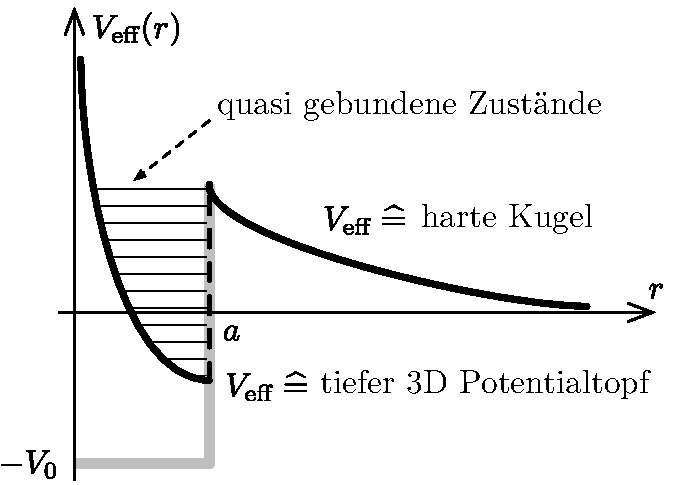
\includegraphics[scale=0.75]{Figs/Veff} 
\end{figure}\vspace{-4ex} 

In linearer Näherung gilt in der Nähe von $E_R$: $\cot(\delta_l)\approx E-E_R/\Gamma_l$. Wobei $\Gamma_l$ einen hier nicht näher bestimmten Faktor darstellt, welcher von der Resonanzenergie $E_R$ abhängt. Es lässt sich damit dann die sogenannte \textbf{Breit-Wigner-Formel} für die partiellen Streuquerschnitte herleiten: 
\begin{eqnarray*}
	\sigma_l(E) &=& \frac{4\pi(2l+1)}{k^2}\cdot \frac{(\Gamma_l/2)^2}{(E-E_r)^2+(\Gamma_l/2)^2}
\end{eqnarray*}
Der totale Streuquerschnitt $\sigma$ ergibt sich dann als $\sigma=\sum_l\sigma_l$. 

%\end{document}